% Figure: Proposed Methodology — 4 phases, 7 stages
% Inline TikZ — vector quality, no external dependencies
%
% Layout: four phase columns side by side with stage boxes inside.
% Horizontal arrows show development flow; dashed arc below shows ITER.

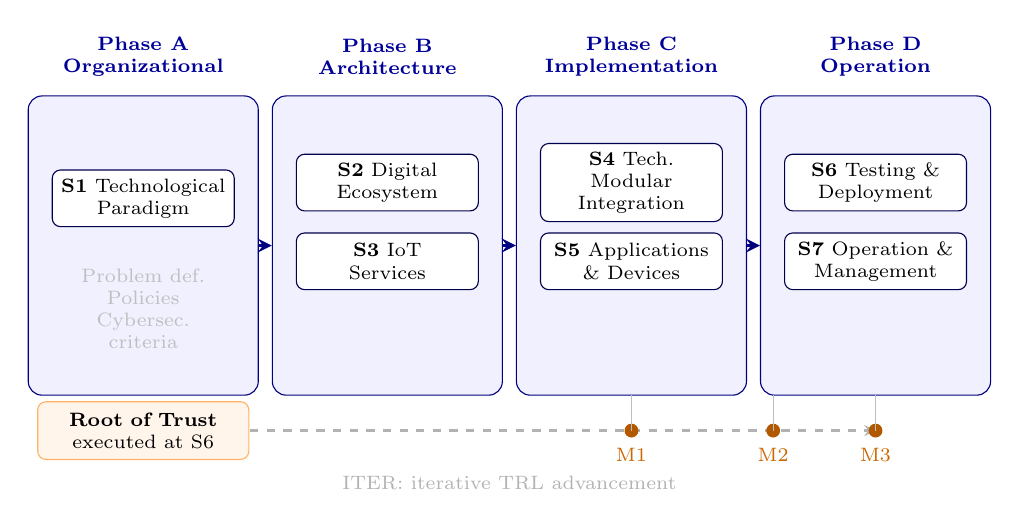
\begin{tikzpicture}[
  font=\small,
  every node/.style={},
  phbox/.style={
    draw=blue!50!black, fill=blue!6, rounded corners=5pt,
    minimum width=2.7cm, text width=2.5cm, minimum height=3.8cm,
    align=center, inner sep=6pt
  },
  phlabel/.style={
    font=\bfseries\scriptsize, text=blue!60!black,
    text width=2.4cm, align=center
  },
  stbox/.style={
    draw=blue!30!black, fill=white, rounded corners=3pt,
    minimum width=2.3cm, text width=2.1cm,
    minimum height=0.72cm, align=center,
    font=\scriptsize, inner sep=3pt
  },
  stno/.style={
    font=\bfseries\scriptsize, text=blue!70!black
  },
  flowarrow/.style={->, very thick, >=stealth, blue!50!black},
  iterarrow/.style={<->, thick, >=stealth, dashed, gray!60},
  maintpt/.style={circle, fill=orange!70!black, minimum size=5pt, inner sep=0}
]

% ── Phase A: Organizational ─────────────────────────────────
\node[phbox] (phA) at (0,0) {};
\node[phlabel] at (0, 2.4) {Phase A\\Organizational};
\node[stbox] at (0, 0.6) {\textbf{S1} Technological\\Paradigm};
\node[font=\scriptsize, text=gray!50, align=center, text width=2.1cm] at (0,-0.8) {Problem def. \\Policies\\Cybersec. criteria};

% ── Phase B: Architecture ───────────────────────────────────
\node[phbox] (phB) at (3.1,0) {};
\node[phlabel] at (3.1, 2.4) {Phase B\\Architecture};
\node[stbox] at (3.1, 0.8) {\textbf{S2} Digital\\Ecosystem};
\node[stbox] at (3.1,-0.2) {\textbf{S3} IoT\\Services};

% ── Phase C: Implementation ─────────────────────────────────
\node[phbox] (phC) at (6.2,0) {};
\node[phlabel] at (6.2, 2.4) {Phase C\\Implementation};
\node[stbox] at (6.2, 0.8) {\textbf{S4} Tech.\ Modular\\Integration};
\node[stbox] at (6.2,-0.2) {\textbf{S5} Applications\\\& Devices};

% ── Phase D: Operation ──────────────────────────────────────
\node[phbox] (phD) at (9.3,0) {};
\node[phlabel] at (9.3, 2.4) {Phase D\\Operation};
\node[stbox] at (9.3, 0.8) {\textbf{S6} Testing \&\\Deployment};
\node[stbox] at (9.3,-0.2) {\textbf{S7} Operation \&\\Management};

% ── Phase flow arrows ────────────────────────────────────────
\draw[flowarrow] (phA.east) -- (phB.west);
\draw[flowarrow] (phB.east) -- (phC.west);
\draw[flowarrow] (phC.east) -- (phD.west);

% ── ITER cycle arc ───────────────────────────────────────────
\draw[iterarrow] (0,-2.35) -- (9.3,-2.35)
    node[pos=0.5, below=0.45cm, font=\scriptsize, text=gray!60] {ITER: iterative TRL advancement};

% ── Maintenance points ───────────────────────────────────────
% M1 fires during implementation (Phase C, x=6.2)
\node[maintpt, label={[font=\scriptsize, text=orange!80!black]below:M1}] at (6.2,-2.35)  {};
% M2 fires during deployment (Phase D, x=8.0)
\node[maintpt, label={[font=\scriptsize, text=orange!80!black]below:M2}] at (8.0,-2.35)  {};
% M3 fires during operation (Phase D, x=9.3)
\node[maintpt, label={[font=\scriptsize, text=orange!80!black]below:M3}] at (9.3,-2.35)  {};

% ── Maintenance point tick lines ─────────────────────────────
\draw[thin, gray!50] (6.2,-1.9) -- (6.2,-2.35);
\draw[thin, gray!50] (8.0,-1.9) -- (8.0,-2.35);
\draw[thin, gray!50] (9.3,-1.9) -- (9.3,-2.35);

% ── RoT highlight note ──────────────────────────────────────
\node[draw=orange!60, fill=orange!8, rounded corners=3pt, font=\scriptsize,
      text width=2.4cm, align=center, inner sep=4pt] at (0,-2.35)
      {\textbf{Root of Trust}\\executed at S6};

\end{tikzpicture}
